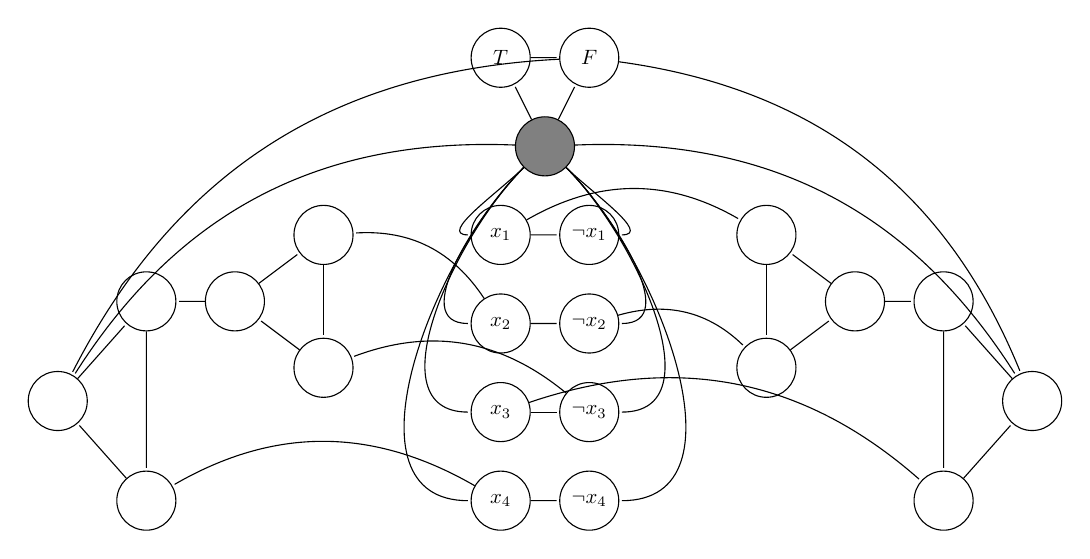
\begin{tikzpicture}[shorten >=1pt,node distance=2cm,auto,scale=1.5,nd/.style={draw=black,circle,scale=\sc,minimum width=0.75 cm,minimum height=1 cm},ndg/.style={nd,fill=gray},scale=0.75]
\def\sc{0.75}
\node[ndg] (R10) at (0.5,3) {};
\node[nd]  (R00) at (0,4)   {$T$};
\node[nd]  (R01) at (1,4)   {$F$};
\foreach \i in {1,...,4} {
  \node[nd]  (V\i0) at (0,3-\i)   {$x_{\i}$};
  \node[nd]  (V\i1) at (1,3-\i)   {$\neg x_{\i}$};
  \path (R10) edge[out=225,in=180] (V\i0);
  \path (R10) edge[out=315,in=0] (V\i1);
  \path (V\i0) edge (V\i1);
}
\foreach \i/\j in {10/00,00/01,10/01} {
  \path (R\i) edge (R\j);
}
\foreach \i/\xa/\ya/\xs/\va/\vb/\vc in {0/3/2/1/10/21/30,0/-2/2/-1/20/31/40} {
  \begin{scope}[xshift=\xa cm, yshift=\ya cm,xscale=\xs]
    \node[nd] (gi\i) at (0,0) {};
    \node[nd] (gj\i) at (0,-1.5) {};
    \node[nd] (gl\i) at (1,-0.75) {};
    \node[nd] (gm\i) at (2,-0.75) {};
    \node[nd] (gn\i) at (2,-3) {};
    \node[nd] (gf\i) at (3,-1.875) {};
    \path (gi\i) edge (gj\i);\path (gj\i) edge (gl\i);\path (gl\i) edge (gi\i);
    \path (gm\i) edge (gn\i);\path (gn\i) edge (gf\i);\path (gf\i) edge (gm\i);
    \path (gl\i) edge (gm\i);
    \path (R10) edge[bend left] (gf\i);
    \path (R01) edge[bend left] (gf\i);
    \path (V\va) edge[bend left] (gi\i);
    \path (V\vb) edge[bend left] (gj\i);
    \path (V\vc) edge[bend left] (gn\i);
  \end{scope}
}
\end{tikzpicture}